En la figura \ref{fig:prob_err} se muestra la probabilidad de error de ambos sistemas en función de la \textit{SNR}, en casos de distintas cantidades de repetidores. Las curvas del sistema analógico se hicieron en base a un $h=1$ (figura \ref{fig:prob_err_a}) y $h=0.5$ (figura \ref{fig:prob_err_b}) para ilustrar la influencia del mismo sobre la probabilidad del error. El error en el sistema digital no depende del valor de $h$.


\begin{figure}[]
    \centering
    \begin{subfigure}[t]{0.8\textwidth}
        \centering
        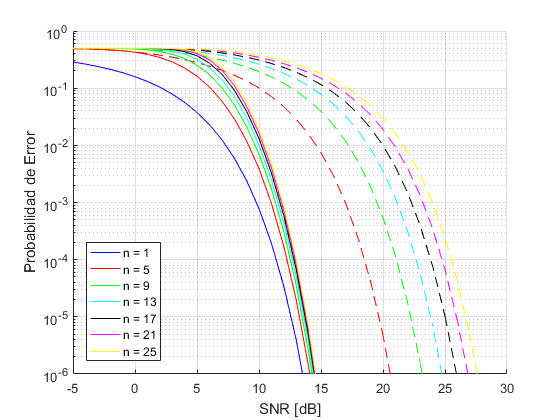
\includegraphics[width=\textwidth]{./Matlab/ej3h=1.png}
        \caption{$h=1$}
        \label{fig:prob_err_a}
    \end{subfigure}%
    \\
    \begin{subfigure}[t]{0.8\textwidth}
        \centering
        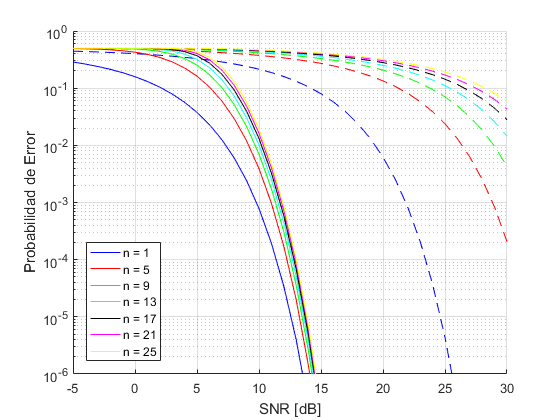
\includegraphics[width=\textwidth]{./Matlab/ej3h=05.png}
        \caption{$h=0.5$}
        \label{fig:prob_err_b}
    \end{subfigure}
    \caption{Probabilidad de error en función del SNR. La línea punteada representa el sistema analógico, y la continua el digital.}
\label{fig:prob_err}
\end{figure}

Para ambos sistemas, independientemente del valor de $h$ y para cada $n$, ocurren cuando $\textbf{SNR}=\SI{-5}{\decibel}$. Mientras menor es el valor de \textbf{SNR} y $n$, más parecido es el error en ambos sistemas (siendo idéntico en el caso en que $n=1$), lo cual resulta claro a partir de las expresiones matemáticas. A su vez, a medida que se tiene un valor menor de $h$, mayor es el error del sistema analógico. 

Teniendo esto en cuenta, resulta evidente elegir el sistema digital, debido a su menor probabilidad de error.

También se observa que al agregar repetidores (valor mayor de $n$), las curvas se abren más, reflejando el agregado de fuentes de ruido. Este hecho resulta más evidente en el caso del sistema analógico. Esto podría deberse en parte al fenómeno de que el error de una etapa digital compense el error de otra. 

La fórmula de probabilidad de error para el sistema digital puede demostrarse a partir de un argumento por recurrencia. Se parte de la fórmula de probabilidad de error para un sistema de un solo repetidor, la cual toma la siguiente forma:

\begin{equation}
P_{e,1}=\mathbb{P}(X_2\neq X_1) 
\end{equation} 

Esta probabilidad es igual a $Q(\sqrt{\textbf{SNR}})$. Si se agrega otro repetidor, se tiene que

\begin{equation}
P_{e,2}=\mathbb{P}(X_3\neq X_1)=\mathbb{P}(X_3\neq X_2)\mathbb{P}(X_2 = X_1)+\mathbb{P}(X_3 = X_2)\mathbb{P}(X_2\neq X_1)
\end{equation} 

lo que equivale a 

\begin{equation}
P_{e,2}=P_{e,1}(1-P_{e,1})+(1-P_{e,1})P_{e,1}
\end{equation} 

dado que $X_2 = X_1$ es complementario al error, y $X_3 \neq X_2$ es probabilidad de error con un solo repetidor. Con esto puede generalizarse que para $n$ repetidores vale

\begin{equation}
P_{e,n}=P_{e,1}+P_{e,n-1}-2P_{e,1}P_{e,n-1}
\end{equation} 

Ahora bien, esto es una ecuación en diferencias con condición inical $P_1 = Q(sqrt{SNR})$. 

Para continuar operando y por comodidad, se llamarán $x[n]=P_{e,1},\alpha=P_{e,1},\beta=1-2P_{e,1}$. Se reescribe la ecuación anterior de la siguiente forma:

\begin{equation}
x[n]-\beta x[n-1]=\alpha
\end{equation} 

con solución de la ecuación homogénea $x_H[n]=k\beta^n$, con $k \in \mathbb{R}$ dependiendo de la condición inicial. Se propone $x_P[n]=c$ como solución particular, con $c\in\mathbb{R}$. Reemplazando, se obtiene que 

\begin{equation}
c=\frac{\alpha}{1-\beta}
\end{equation} 

Sumando ambas soluciones para obtener la solución a la ecuación, y con la condición inicial, se obtiene que 

\begin{equation}
k = \frac{P_{e,1}}{\beta}-\frac{\alpha}{\beta-\beta^2}
\end{equation} 

Siendo entonces la solución

\begin{equation}
x[n]=(\frac{P_{e,1}}{\beta}-\frac{\alpha}{\beta-\beta^2})\beta^n+\frac{\alpha}{1+\beta}
\end{equation} 

Finalmente, reemplazando los valores de $\alpha,\beta,P_{e,1}$ se llega a la expresión de probabilidad de error para un sistema digital

\begin{equation}
P_{e,n}=\frac{1}{2}(1-(1-2Q(\sqrt{\textbf{SNR}})^n))
\end{equation} 